\section{Desenvolvimento}

%TODO : revisar esta parte com a Ceci


A partir dos resultados obtidos na pesquisa o próximo passo do trabalho foi planejar e desenvolver um sistema com o objetivo de auxiliar os times ágeis nas suas reuniões de melhoria contínua.

O levantamento dos requisitos foi feito em meados de agosto e a implementação da aplicação ocorreu de setembro até novembro. O código do projeto está em um repositório do GitHub~\footnote{https://github.com/mxball/suricato}.

\subsection{Planejamento}

%está ruim
A pesquisa gerou conhecimentos empíricos sobre os problemas enfrentados na promoção de melhoria contínua. O planejamento da aplicação pode-se resumir a algumas metas a serem alcançadas: (i)Desenvolver a lousa virtual, (ii)guardar as informações dos usuários, (iii)subir o sistema web, e (iv)layout satisfatório.

%O planejamento da aplicação ocorreu de meados de agosto até o começo de setembro. Como o objetivo da aplicação é ajudar qualquer tipo de equipe, seja local ou distribuído, uma das necessidades é que a aplicação seja acessível pelas máquinas de todos os integrante, independente de sistema operacional. Portanto a opção foi desenvolver uma aplicação web, já que o usuário consegue acessar o sistema através de qualquer navegador.

\subsection{Requisitos do sistema}

%LUCAS: o Planejamento já fala algumas das coisas desses dois parágrafos
Os resultados da pesquisa serviram como base para os requisitos do sistema. Nota-se que a grande maioria dos times ainda fazem retrospectivas, com exceção dos times distribuídos em diversos fusos horários. Esses times utilizam reuniões parecidas com retrospectivas, como, por exemplo, as \textit{conference calls}. A única diferença é que elas não seguem uma estrutura como a retrospectiva, como a apresentada por Derby e Larsen~\cite{retrospectives}. 

Os requisitos da aplicação foram baseados na forma como a retrospectiva é feita localmente. No entanto, ela não exige que o time siga o seu fluxo predefinido, como outras aplicações encontradas no mercado obrigam, por exemplo, a Retrium~\footnote{https://retrium.com/}.

\subsubsection*{Lousa virtual}

Em geral, a forma como as retrospectivas são feitas por times locais é utilizando um quadro branco, post-its e canetas. No começo da reunião o facilitador apresenta no quadro algum formato de retrospectiva, também conhecido como atividade. Depois de explicar a atividade para as pessoas, cada integrante pode colocar na lousa post-its, dando suas opiniões, apontando problemas no time, entre outros. A partir dos post-its o time consegue discutir e gerar ideias sobre como melhorar. Cada uma das ideias são escritas na lousa ou em post-its. Por fim, o time escolhe as melhores e define ações que o serão adotadas pela equipe para implementá-la. Essas ações também podem ser escritas na lousa ou em post-its.

O primeiro requisito era que o usuário pudesse criar uma lousa virtual. Escolhendo um formato de retrospectiva e o sistema gera uma tela como um quadro branco com a atividade escolhida desenhada no fundo.

A lousa virtual deve permitir todas as facilidades que a lousa real. Nesse sentido, as funcionalidades de adicionar post-its e escrever comentários na tela foram implementados. Para gerar uma maior usabilidade da aplicação, foram adicionados post-its de diferentes cores, remoção e edição dos post-its e comentários da tela.

\subsubsection*{Falta de engajamento e discussões de pouco valor}

Os desafios mais citados pelos times que fazem a retrospectiva foram a falta de engajamento das pessoas e as discussões de pouco valor. Poussard~\cite{poussard} aponta que um dos costumes que times ágeis tem é que muitos acabam criando hábitos nas retrospectivas e executando sempre os mesmos tipos de atividades. Ele defende que isso acaba enfraquecendo a evolução que poderia ser conquistada. Segundo Derby e Larsen~\cite{retrospectives},  as pessoas tendem a perder o interesse na retrospectiva quando estão fazendo sempre as mesmas atividades.

Para investigar os pontos levantados nesses artigos, foi adicionada uma pergunta a ser respondida apenas por times que fazem retrospectivas sobre a alternância de atividades nessa reunião e, em caso positivo, quais são as atividades mais utilizadas. As repostas não foram conclusivas, mas geraram a hipótese de que os times variam as atividades mas não o tipo da atividade. Das retrospectivas citadas pelos times que responderam sim, a maior parte delas eram do formato de encontrar problemas e discutir soluções. 

A pesquisa não foi suficiente para contrapor os artigos, foi adicionado os requisitos que incentivam os usuários a variar seus tipos de atividades. Para isso, o sistema deveria conter uma listagem com os mais diversos formatos de atividades para o usuário escolher. A apresentação das diversas opções pode ajudar os times a conhecerem novas retrospectivas e alternar entre os diversos tipos. Isso pode resolver os  problemas de falta de engajamento das pessoas e as discussões pouco produtivas.

\subsubsection*{Tempo real}

Como os times são formados por um conjunto de pessoas e como elas podem estar espalhados por diversas regiões, um dos principais requisitos definidos é que todos os integrantes devem mexer na mesma lousa virtual. As lousas foram planejadas  para funcionarem em tempo real para muitos usuários, ou seja, todos os usuários estão visualizando a mesma lousa e tudo que for alterado por alguma pessoa será mostrado no navegador dos outros integrantes.

\subsubsection*{\textit{Dot voting} (votação nas opções preferidas)}

Outra dificuldade que foi muito citada na pesquisa é ultrapassar a duração da reunião. Uma das causas desse problema é que durante a coleta dos dados, como cada integrante vai adicionar os seus post-its, a quantidade de dados acaba sendo muito grande. Muitas equipes decidem discutir todos os pontos levantados e acabam estourando o tempo definido para a reunião.

Na retrospectiva, uma das formas de reduzir o número de post-its que serão discutidos é encontrar quais são os pontos mais relevantes para se discutir. Para isso cada integrante vota nos post-its que ele considera mais importantes e somente os mais votados serão discutidos na reunião. Essa forma de filtrar os dados é conhecida nas retrospectivas como \textit{dot voting}.

Por se tratar de uma técnica eficiente de diminuir o tempo da reunião e influenciar o time a debater o que é mais essencial, foi decidido que o sistema deve possibilitar essa votação. Mesmo sendo um recurso específico da retrospectiva, ele pode ajudar inclusive os times que realizam outras reuniões de melhoria contínua. Cada um dos votos que o post-it recebe é marcado na tela, assim os integrantes podem indicar quais são os mais relevantes.

\subsection{Trello}

Para organizar os requisitos e todos os participantes do projeto saberem o que estava sendo implementado, o sistema usado para gerenciar o trabalho foi o Trello. Para cada um dos requisitos são criados cartões que definem o que será implementado.

\begin{figure}[H]
  \hspace*{-4em}
  \fbox{
    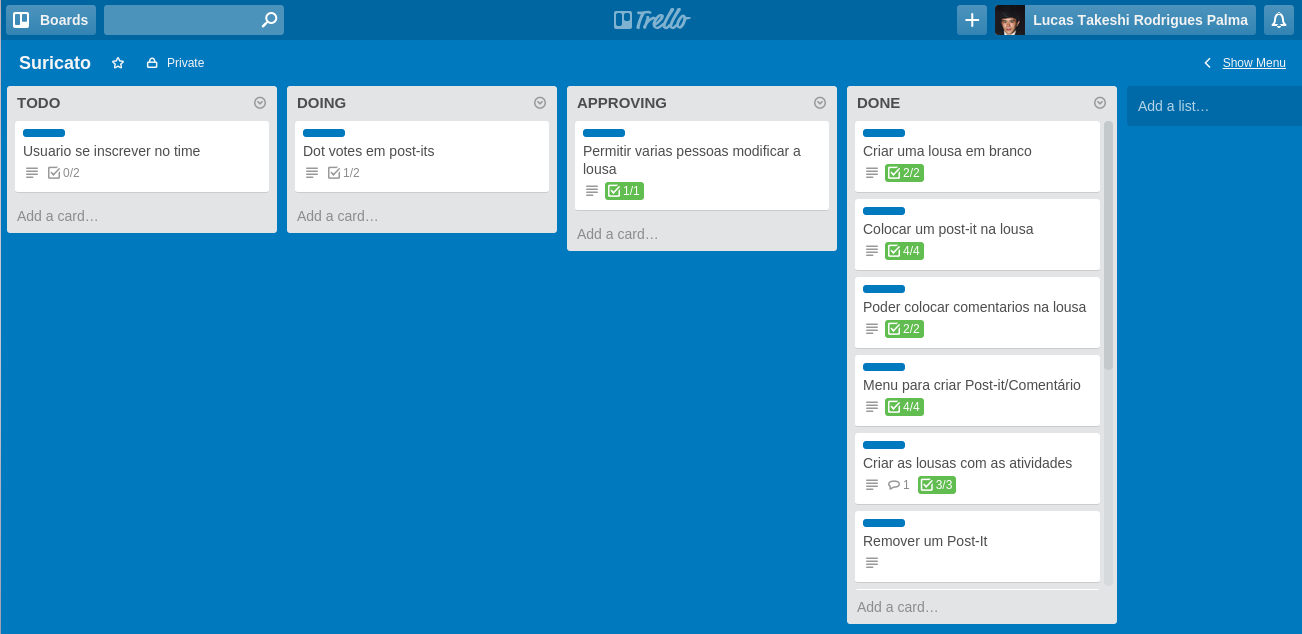
\includegraphics[width=170mm]{images/requisitos.png}
  }
  \caption{Requisitos do sistema}\label{figura:requisitos}
\end{figure}

Cada um desses cartões segue os modelos de cartões de história da agilidade, em que são dadas três informações:

\begin{itemize}
	\item Para: por que é importante que o sistema tenha essa funcionalidade
	\item Como: que tipo de usuário se beneficia mais com essa funcionalidade
	\item Quero: objetivamente, o que se quer que o software faça
\end{itemize}

\begin{figure}[H]
  \hspace*{-4em}
  \fbox{
    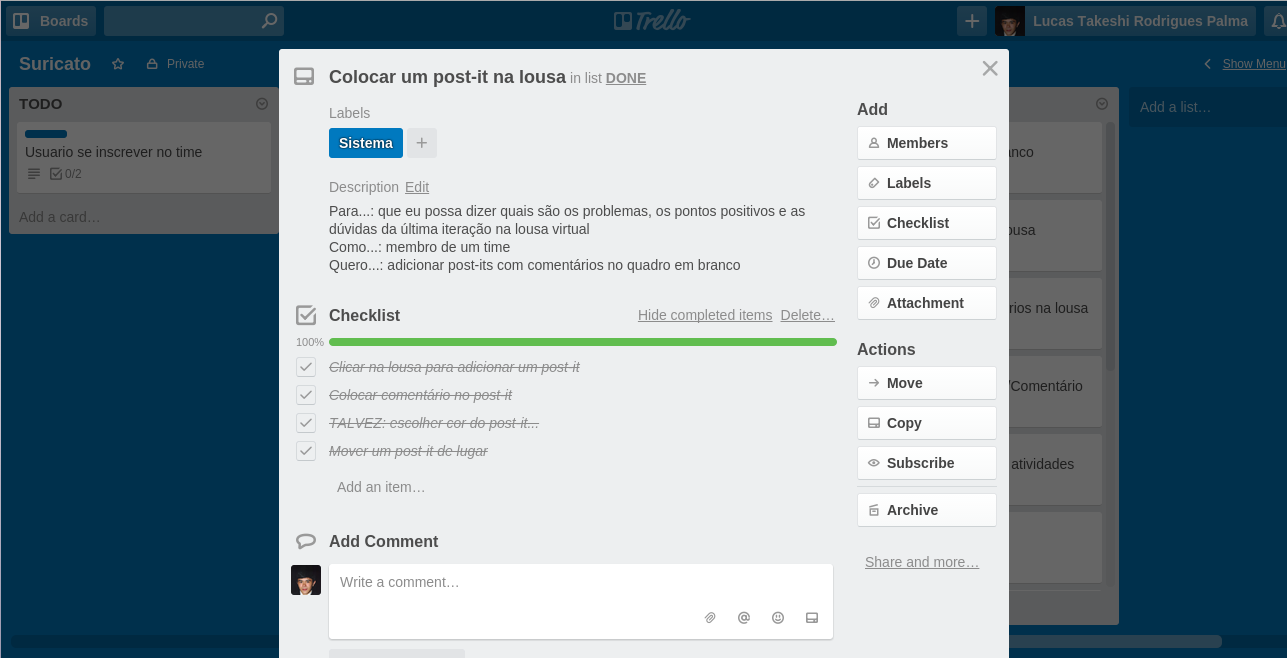
\includegraphics[width=170mm]{images/cartaoHistoria.png}
  }
  \caption{Modelo de cartão de história}\label{figura:cartao}
\end{figure}

\subsection{Tecnologias e criação do projeto}

Para o desenvolvimento da aplicação a linguagem escolhdia foi o Java. Em conjunto com a linguagem foram utilizadas as tecnologias a seguir.

\subsubsection*{Framework MVC}

Hoje em dia, uma das formas mais utilizadas no mercado para desenvolver aplicações web é através da arquitetura MVC (\textit{Model View Controller}), na qual seu sistema é dividido em três partes:

\begin{itemize}
	\item \textit{Models}: classes que representam as entidades do sistema (por exemplo, usuário e time) e as que ajudam a armazenar e buscar os dados.
	\item \textit{Views}: responsável por apresentar os resultados na página web.
	\item \textit{Controllers}: responsável por processar as requisições, instanciar os modelos necessários para realizar a tarefa requisitada e chamar as \textit{views}.
\end{itemize}

Existem diversos \textit{frameworks} no mercado que seguem essa estrutura e o escolhido para desenvolver o TCC foi o Spring MVC.

\subsubsection*{Autenticação e Autorização}

Como um dos requisitos do sistema é que uma pessoa possa criar uma lousa virtual e todos os integrantes do seu time possam participar da reunião através da mesma lousa, uma das necessidades do sistema é que o usuário se identifique através de um usuário (autenticação) e quando ele tentar acessar alguma tela o sistema verifique se ele possui permissão (autorização).

Já existem diversas bibliotecas no mercado que abstraem as lógicas de autenticação e autorização, sendo necessário apenas informar qual o modelo de usuário usado pelo sistema. O \textit{framework} escolhido foi o Spring Security devido à facilidade de integração com o Spring MVC.
%REVISAR A SUBSECAO
\subsubsection*{Banco de dados}

%LUCAS: Essa linha vai sumir ne?
Desde o início do projeto houve a necessidade de algum banco para guardar os seus dados, como, por exemplo, os usuários, lousas virtuais, entre outros. A base de dados usada é o MySQL.

%LUCAS (Sugestão para a primeira frase): Como o sistema trabalha com diversas informações, como os usuários e as lousas virtuais, ele precisa se integrar com algum banco para armazenar seus dados. 
O sistema ainda precisava se integrar com o banco para conseguir armazenar seus dados. Como o sistema  está escrito na linguagem Java, cujo paradigma é a Orientação a Objetos, enquanto os bancos de dados SQL seguem o paradigma Relacional, existe uma barreira de comunicação entre eles.

Já existem diversos \textit{frameworks} no mercado que abstraem essa comunicação entre as aplicações orientadas a objetos e bancos relacionais, conhecidos como ORM (\textit{Object-relational Mapping}). O mais utilizado é o Hibernate e foi a escolha para o projeto.
%REVISAR A SUBSECAO
\subsubsection*{Servidor de aplicação e WebSockets}

Por se tratar de uma aplicação web, é essencial escolher em qual servidor rodará o sistema pois um dos requisitos do mesmo é possuir lousas que possam ser acessadas por vários usuários e as alterações devem ser em tempo real. Uma das formas conhecidas para fazer essa funcionalidade é usar o conceito de WebSockets -- um protocolo de redes que estabelece como criar um canal de comunicação entre o navegador e o servidor.

Toda vez que um usuário acessar uma lousa virtual é criado um canal com o servidor, conhecido como socket. Através dele o navegador consegue enviar mensagens para o servidor informando todas as ações feitas pelo usuário, como a de adicionar um post-it, editar um comentário, entre outros. Quando o servidor receber essa mensagem, ele armazena no banco essa informação e a retransmite para todos os sockets que ele possui. Cada integrante que está acessando a lousa virtual recebe a mensagem através do socket informando alguma alteração feita por outra pessoa e consegue reproduzi-la na sua tela.

O WebSockets ainda é recente e não são todos os servidores de aplicação que possuem suporte nativo para esse protocolo. Por isso o servidor escolhido foi o WildFly, desenvolvido pela RedHat, que já possui suporte.

\subsubsection*{Nascimento do Suricato}

Uma das partes mais complicadas no começo de um grande projeto web é a integração entres os diversos \textit{frameworks} que serão usados. Isso envolve muitas horas escrevendo diversos arquivos de configuração, em geral arquivos XML (Extensible Markup Language). Mesmo programadores com mais experiência levam longas horas até que todas as configurações fiquem corretas. 

A integração seria entre os \textit{frameworks} Spring MVC, Spring Security e Hibernate. Para não ocupar muito tempo com a configuração, o projeto foi gerado através do site Setup My Project~\footnote{http://www.setupmyproject.com/}. Ele permite que uma pessoa escolha quais tecnologias seu projeto usará e gera automaticamente uma versão simples de um sistema com todos os \textit{frameworks} escolhidos já configurados.

%LUCAS: Na subsecao anterior já foi explicado essa parte do porque escolher o wildfly. Acho que essa linha pode ser apagada
Para a aplicação ficar no ar era necessário configurar um servidor de aplicação. Foi escolhido o WildFly, por ser mais compatível com a tecnologia de WebSocket.

Devido uma antiga tradição no IME de que os projetos do instituto recebem o nome de animais, a inspiração veio em procurar algum animal que saiba trabalhar bem em equipe. Assim, o sistema do Suricato nasceu.

\subsubsection*{Dificuldades de integração WildFly, WebSockets e Spring MVC}

Com os \textit{frameworks} configurados, faltava habilitar o WebSocket implementado pelo WildFly para funcionar com o Spring MVC.

A classe criada no sistema responsável por criar e utilizar o WebSocket do lado do servidor é a RetrospectivaEndpoint. Para marcá-la como uma classe do WebSocket basta anotar a classe com um @ServerEndpoint e passar qual a url pela qual o canal de comunicação será criado.

Bastaria que esta classe armazenasse as informações recebidas através do \textit{socket} no banco de dados. Todos os códigos usados para comunicação com o banco foram isolados em classes que seguem o padrão de projeto DAO~\footnote{http://www.oracle.com/technetwork/java/dataaccessobject-138824.html}. Por trabalhar com o Spring MVC, as classes DAO são anotadas com o @Repository. Com esta anotação, quem passa a gerenciar a classe -- cria objetos a partir dela e distribui esses objetos para outras classes que precisam usá-la -- é o Spring MVC. Esta forma de trabalhar do \textit{framework} segue dois padrões de projeto, o Inversion of Control Containers e a Dependency Injection~\footnote{http://www.martinfowler.com/articles/injection.html}.

%REVISAR OS PROXIMOS DOIS PARAGRAFOS
Então o cenário do sistema é que havia a classe RetrospectivaEndpoint, gerenciada pelo servidor de aplicação WildFly. Esta classe precisava receber objetos DAO's para enviar as informações para o banco de dados, mas estes são gerenciados pelo Spring MVC. O problema é que as duas tecnologias não são capazes de enviar objetos que uma delas está gerenciando para a outra.

Mesmo pesquisando em blogs e fóruns se existiam outras pessoas que já passaram por esse problema de integração e como elas resolveram, nenhuma informação foi encontrada. Depois de algum tempo estudando mais a fundo as tecnologias e com a ajuda de pessoas da Caelum surgiu uma solução. O Spring MVC possui uma classe chamada de ApplicationContext, que possui objetos de todas as classes que ele gerencia, como os DAO's. Bastava criar a classe auxiliar ApplicationContextHolder, gerenciado pelo Spring e que possui um atributo estático que guarda um objeto de ApplicationContext. Por ser estático, qualquer outra classe do projeto pode acessá-lo, independente de qual tecnologia a gerencia. Assim, a classe RetrospectivaEndpoint consegue receber uma instância de ApplicationContext e, consequentemente, ao DAO.

Esta solução para o problema de integrar o WebSockets do servidor de aplicação WildFly com o \textit{framework} Spring MVC foi publicado no blog Domine o Spring~\footnote{https://domineospring.wordpress.com/2015/11/03/um-pouco-de-gambi-nao-faz-mal-a-ninguem-spring-em-ambientes-nao-gerenciados/}. 

\subsection{Testes do software}

O sistema já tinha as funcionalidades mínimas para ser utilizável. Um usuário consegue criar a lousa, escolher entre diversas atividades para a reunião e adicionar, remover ou editar um post-it ou comentário. Faltava adicionar a autenticação e autorização, deixar a lousa funcionando em tempo real e os \textit{dot voting}.

Antes de implementar estes requisitos, o sistema foi utilizado em equipes pequenas para receber feedbacks. Diversos testes das funcionalidades foram feitos e, consequentemente, alguns bugs foram encontrados.

Para corrigir esses erros, surgiram novas funcionalidades:

\begin{enumerate}
	\item o usuário pode regular o tamanho de um comentário e o tamanho dos post-its é fixo.
	\item comentários sempre aparecem por cima de um post-it.
	\item no campo de texto que deve ser preenchido ao criar o post-it ou comentário, a tecla Enter insere o elemento na tela e o Shift + Enter pula uma linha.
\end{enumerate}

\subsubsection*{Layout}
O Suricato ainda tinha problemas de layout. 

\begin{figure}[H]
  \centering
  \fbox{
    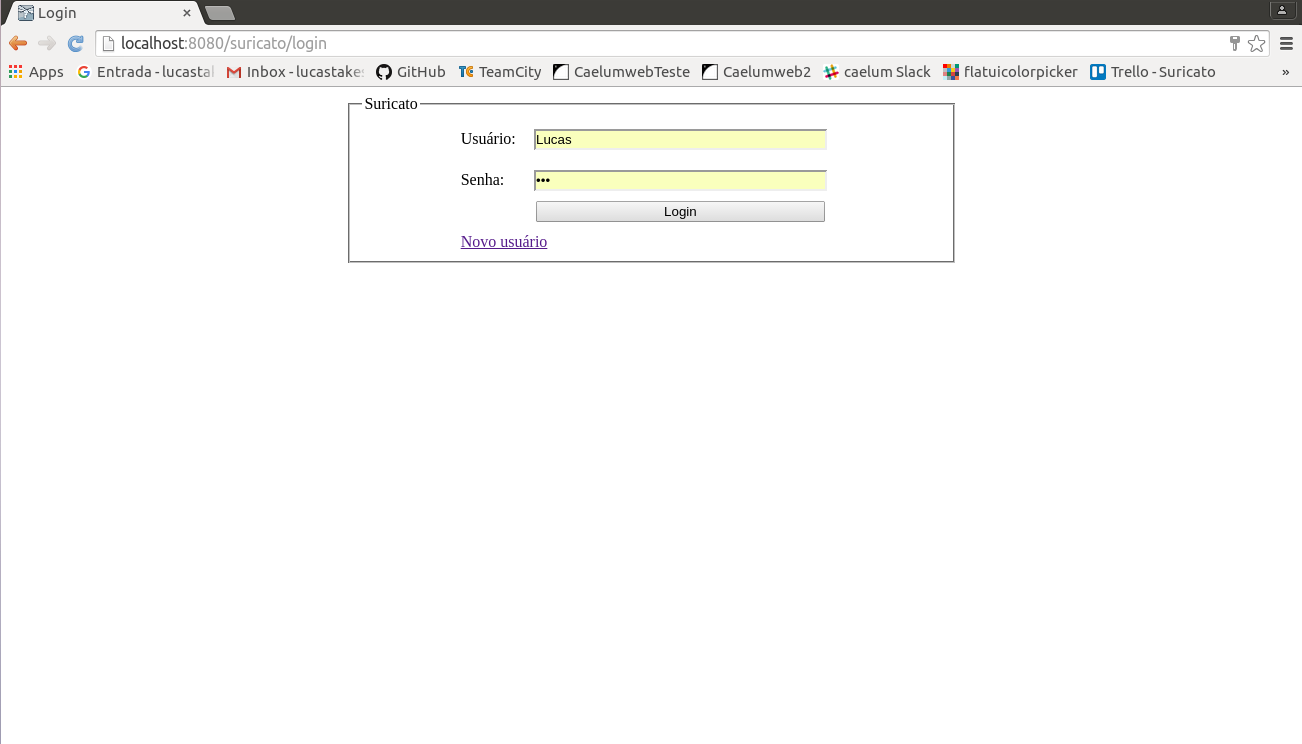
\includegraphics[width=130mm]{images/login.png}
  }
  \caption{Tela antiga de login}\label{figura:loginAntigo}
\end{figure}

\begin{figure}[H]
  \centering
  \fbox{
    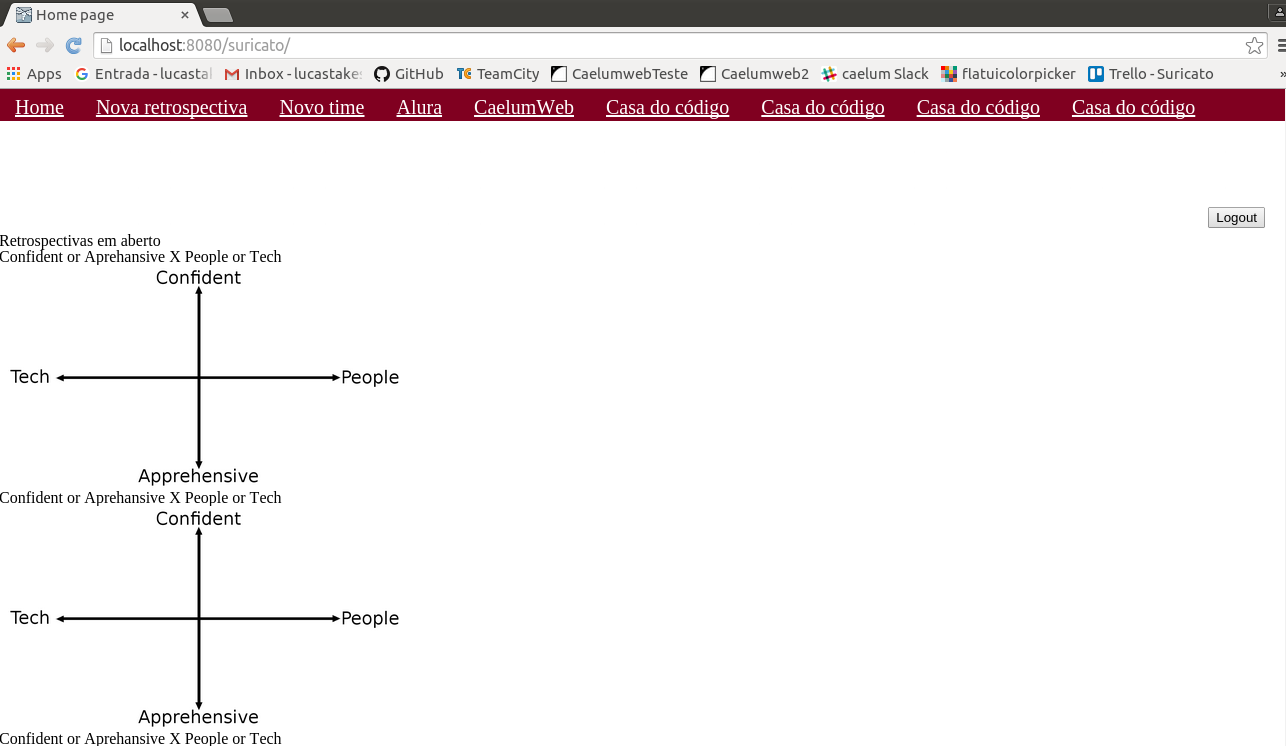
\includegraphics[width=130mm]{images/index.png}
  }
  \caption{Tela antiga do usuário}\label{figura:indexAntigo}
\end{figure}

\begin{figure}[H]
  \centering
  \fbox{
    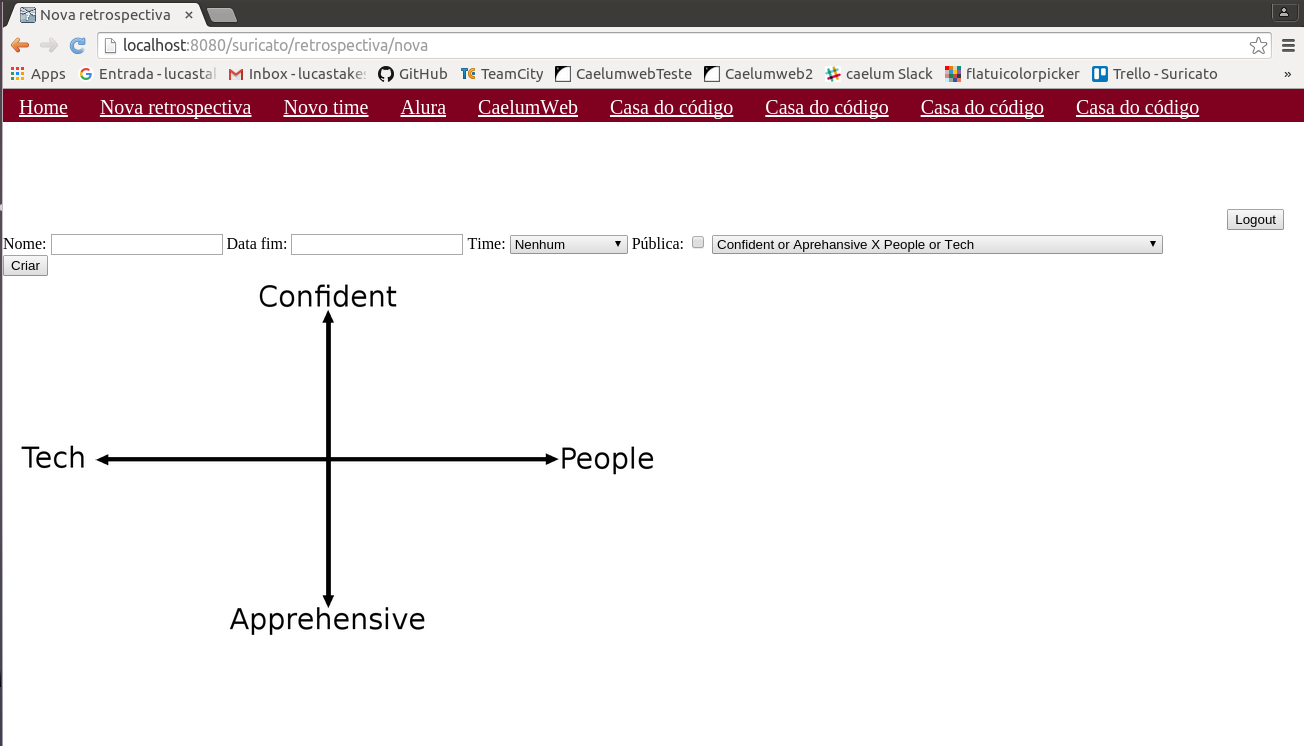
\includegraphics[width=130mm]{images/criar.png}
  }
  \caption{Tela antiga para criar lousa virtual}\label{figura:criarAntigo}
\end{figure}

Para liberar o sistema era necessário planejar um layout. O designer Fabio Gushiken foi o responsável por desenhar o logo baseado no suricato. Algumas atividades era necessário fazer o desenho de fundo da lousa virtual, o designer Leonardo Guerra colaborou com as atividades de Speed Car e Hot Air Balloon. Para melhorar a usabilidade do sistema o instutor Marco Bruno planejou o fluxo que um usuário do sistema poderia seguir e remodelou as telas pensando nesse fluxo.

\begin{figure}[H]
  \centering
  \fbox{
    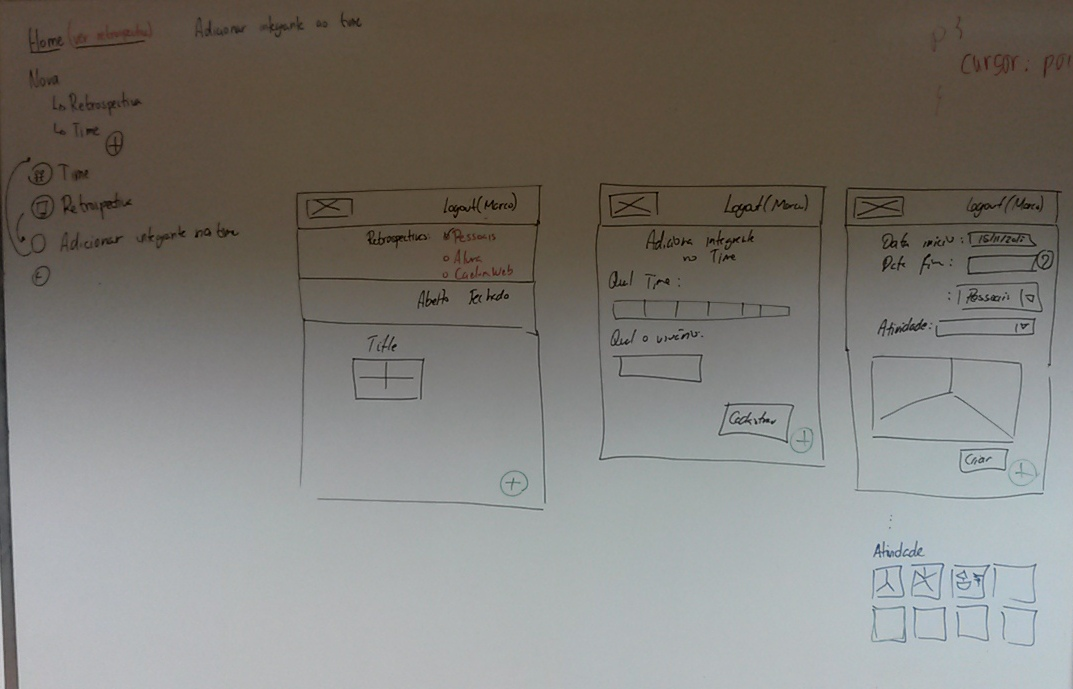
\includegraphics[width=140mm]{images/ux.jpg}
  }
  \caption{Modelagem das telas com UX}\label{figura:ux}
\end{figure}

Para arrumar o layout o foco foi desenvolver as páginas seguindo o que foi planejado na reunião. Abaixo o resultado final:

\begin{figure}[H]
  \centering
  \fbox{
    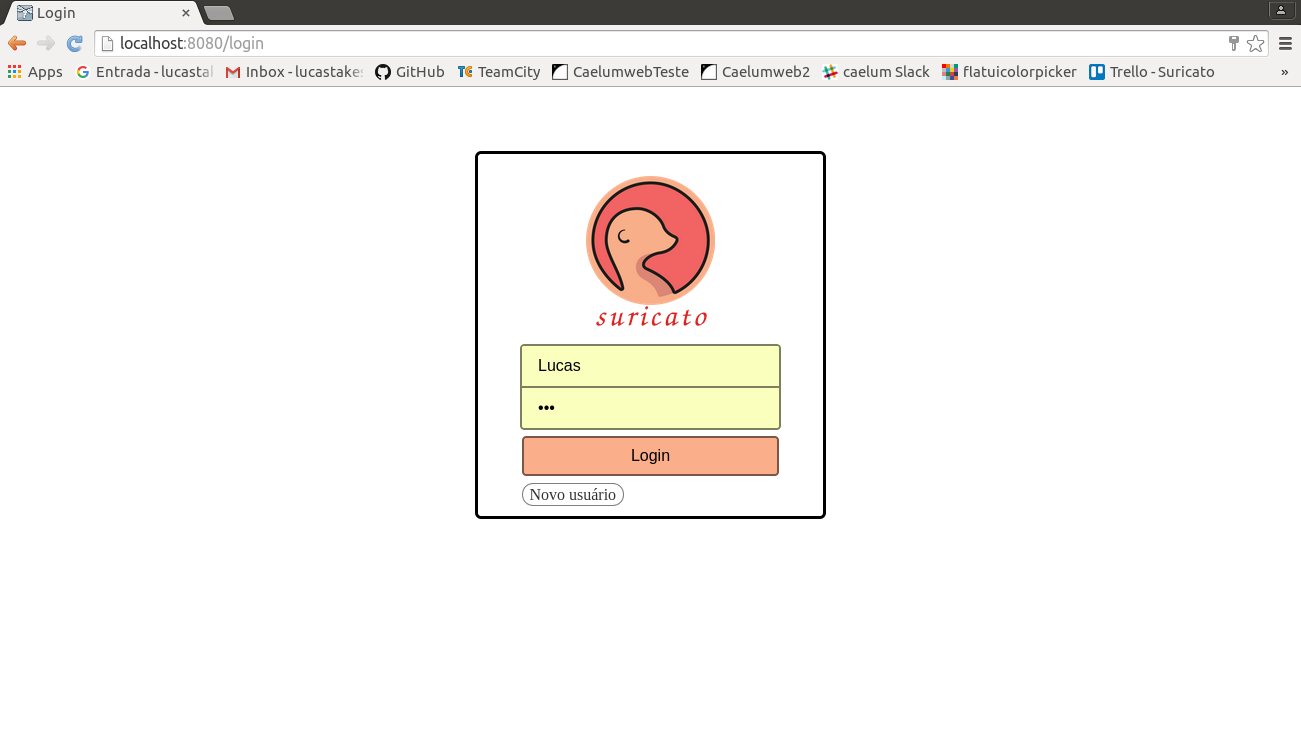
\includegraphics[width=130mm]{images/login2.png}
  }
  \caption{Tela nova de login}\label{figura:loginNovo}
\end{figure}

\begin{figure}[H]
  \centering
  \fbox{
    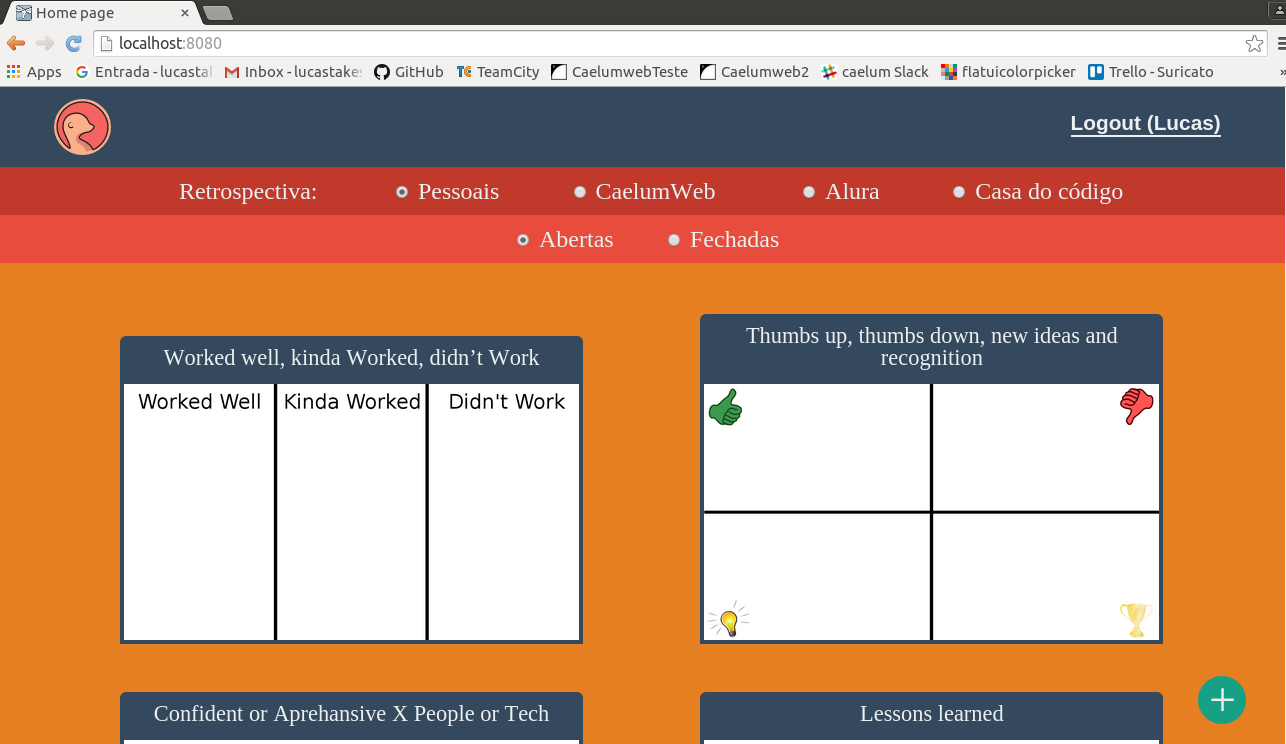
\includegraphics[width=130mm]{images/index2.png}
  }
  \caption{Tela nova do usuário}\label{figura:indexNovo}
\end{figure}

\begin{figure}[H]
  \centering
  \fbox{
    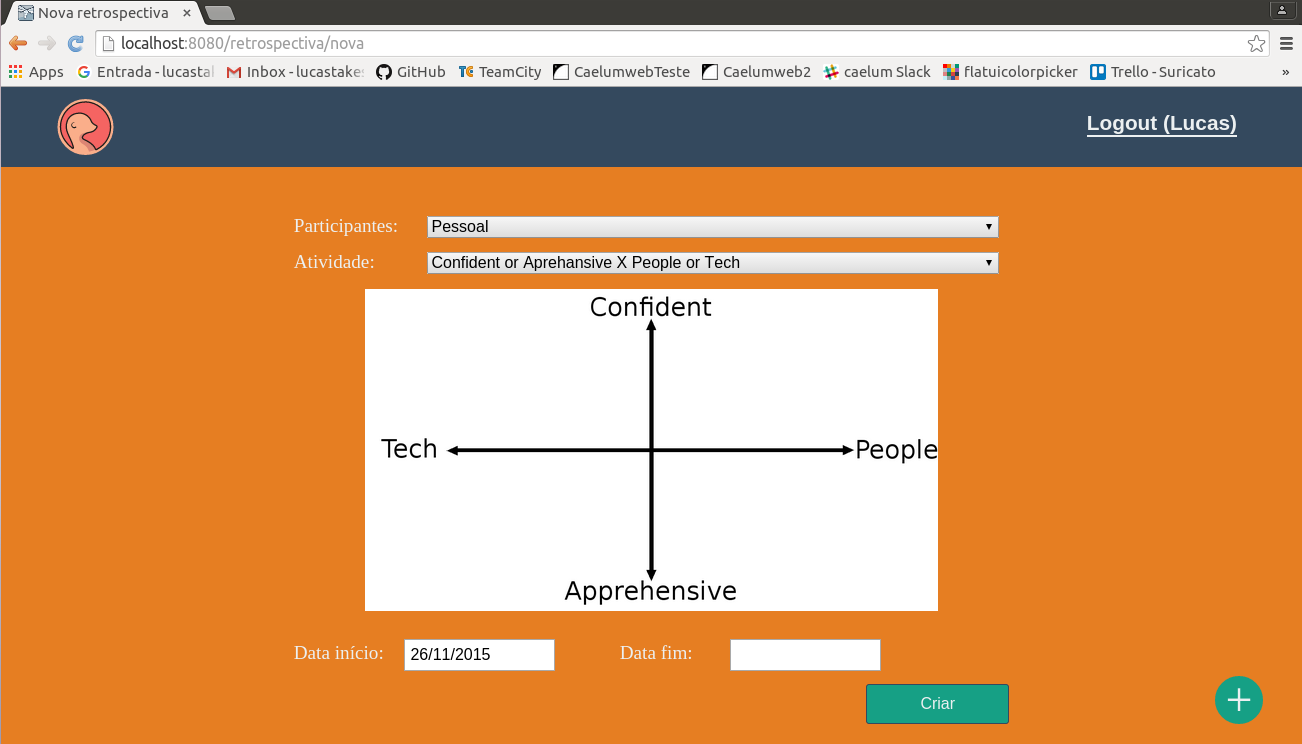
\includegraphics[width=130mm]{images/criar2.png}
  }
  \caption{Tela nova para criar lousa virtual}\label{figura:criarNovo}
\end{figure}

\begin{figure}[H]
  \centering
  \fbox{
    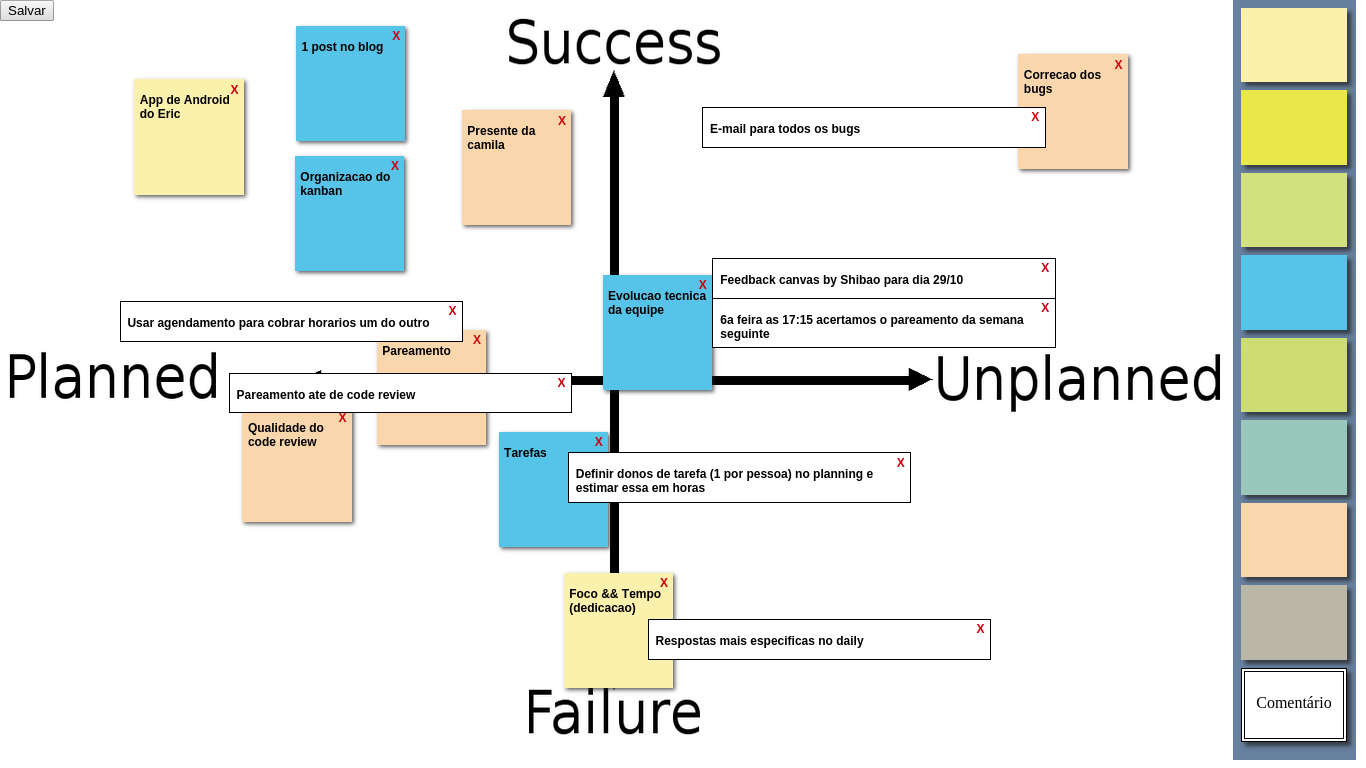
\includegraphics[width=130mm]{images/retrospectiva.png}
  }
  \caption{Tela da lousa virtual}\label{figura:Retrospectiva}
\end{figure}
%Falta
\subsection{Hospedagem}

Com a primeira versão do sistema pronta, faltava apenas hospedar o site. Como o servidor de aplicação era o WildFly da RedHat, a primeira opção foi usar o serviço da Openshift~\footnote{https://www.openshift.com/}, também da RedHat. Essa plataforma permite que qualquer pessoa hospede de graça sua aplicação web e possui máquinas preparadas para usar o WildFly. Por ser gratuito, o Openshift desliga a máquina quando ninguém está usando o sistema e liga quando um usuário tenta acessá-la. No entanto, para o Suricato as máquinas se mostraram muito instáveis, já que depois de ligá-la o sistema não era colocado no ar automaticamente. Alguém precisava se conectar via ssh na máquina e rodar comandos para que o projeto subisse.

Devido a instabilidade da Openshift, tempos depois o sistema foi hospedado na Amazon Web Services~\footnote{https://aws.amazon.com/}. Mesmo levando alguns dias para criar a máquina e preparar o ambiente para rodar com o WildFly, o serviço é bem mais confiável e estável.

Atualmente o domínio usado para acessar o projeto é http://suricatoagil.com/login.